% Adapted from "Resume Template by Krishna Priyatham Potluri"
% (Overleaf, CC BY 4.0). Content and local class customized for Sieun Park.
\documentclass{resume}

\begin{document}

\noindent
\begin{tabularx}{\linewidth}{@{}X >{\raggedleft\arraybackslash}m{2.85cm}@{}}
  {%
    {\LARGE\bfseries Sieun Park}\par
    \vspace{0.25em}
    {\large Mobile Systems Researcher}\par
    \vspace{0.15em}
    {\small AI Privacy \textbar{} Accountable Mobile AI}\par
    \vspace{0.55em}
    {\small\color{muted}
      Seoul, South Korea \textbf{\textperiodcentered}\
      \href{mailto:sieun.park@hcs.snu.ac.kr}{sieun.park@hcs.snu.ac.kr} \textbf{\textperiodcentered}\
      \href{tel:+821059622446}{+82 10-5962-2446}\par
      \href{https://cherry-0.github.io/sieunpark-at-snu/}{cherry-0.github.io/sieunpark-at-snu} \textbf{\textperiodcentered}\
      \href{https://www.linkedin.com/in/sieunpark-at-snu/}{LinkedIn}
    }
  }
  & 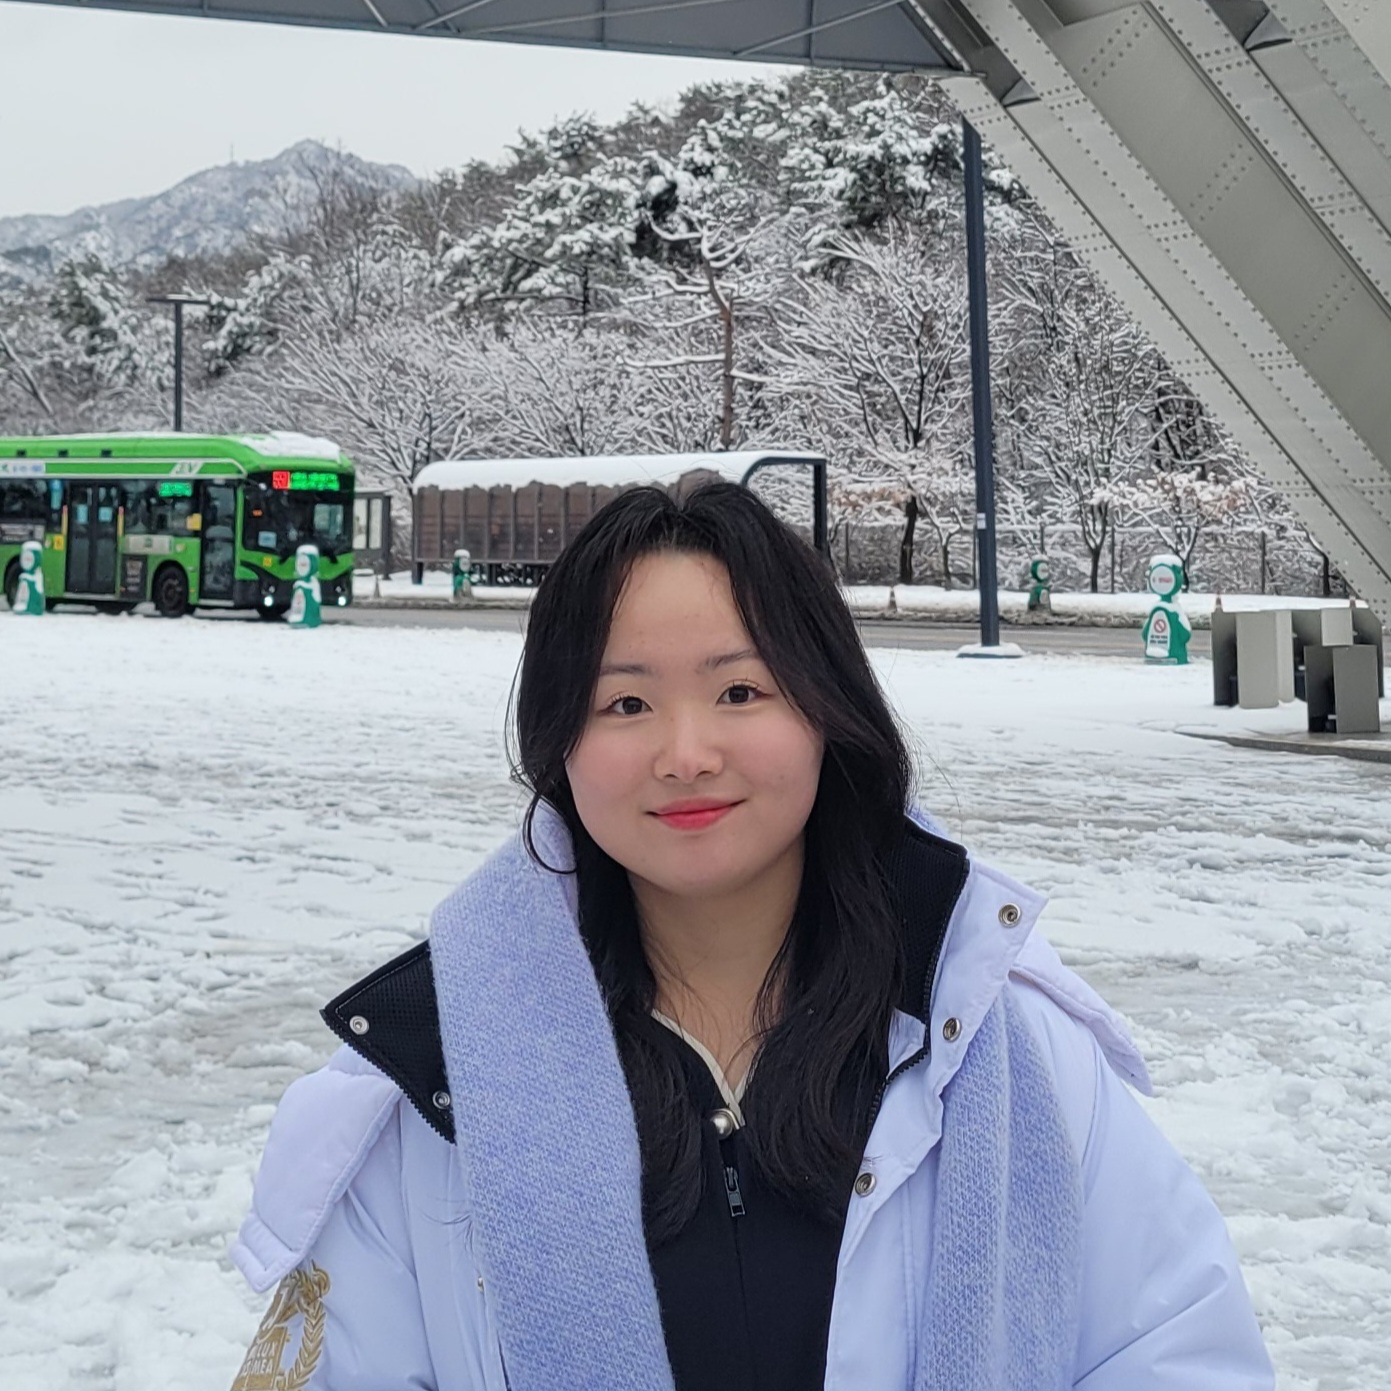
\includegraphics[width=2.8cm]{id_photo.png}
\end{tabularx}

\csection{Summary}{\small
  Mobile systems researcher studying privacy and accountability in LLM/VLM-enabled apps. I characterize how model-derived private attributes propagate through real app workflows and design attribute-, workflow-, and channel-level protections. Earlier work spans AI scaffolding for parent--child storytelling and cross-spatial interaction.
}

\csection{Education}{\small
  \resumeentry{M.S./Ph.D. in Artificial Intelligence}{Sept 2024 -- Present}{Seoul National University}{Seoul, South Korea}
  \vspace{0.35em}
  \resumeentry{B.S. in Mathematics Education \& Artificial Intelligence}{Mar 2018 -- Feb 2024}{Seoul National University}{Seoul, South Korea}
}

\csection{Research Experience}{\small
  \resumeentry{Graduate Researcher}{Sept 2024 -- Present}{Human-Centered Computer Systems Lab, Seoul National University}{Seoul, South Korea}
  \begin{itemize}
    \item Conduct research on mobile AI privacy and accountable mobile systems, focusing on how LLM/VLM-enabled apps infer and expose private attributes in real app workflows.
    \item Characterize how model-derived attributes travel through UI, storage, network, voice, and cross-app channels, and develop attribute-, workflow-, and channel-level privacy protections.
  \end{itemize}

}

\csection{Teaching Experience}{\small
  \resumeentry{Head Teaching Assistant, Software Development Principles and Practices}{Sept 2026 -- Dec 2026}{Seoul National University}{Seoul, South Korea}

  \vspace{0.35em}
  \resumeentry{Teaching Assistant, Software Development Principles and Practices}{Sept 2025 -- Dec 2025}{Seoul National University}{Seoul, South Korea}
  \begin{itemize}
    \item Supported programming assignments, code reviews, and team-based software projects.
  \end{itemize}

  \vspace{0.25em}
  \resumeentry{Teaching Assistant, Education and Artificial Intelligence}{Mar 2023 -- Jun 2023}{Seoul National University}{Seoul, South Korea}
  \begin{itemize}
    \item Mentored project teams designing AI-driven educational applications and provided feedback on technical implementation and pedagogical grounding.
  \end{itemize}
}

\csection{Publications}{\small
  \publicationentry
    {TaleTrain: AI Scaffolding for Parent--Child Video Story Retelling at Home}
    {Sangwon Park, \textbf{Sieun Park}, HyunA Seo, Minkyu Shim, Youngki Lee}
    {Under Review}
  \vspace{0.35em}
  \publicationentry
    {ODFuse: Reducing Reasoning Overhead in Tool-Use Agents via Observation-Dependency-Guided Fusion}
    {Hyunwoo Jung, \textbf{Sieun Park}, Minkyu Shim, Youngki Lee}
    {Under Review}
}

\csection{Presentations}{\small
  \presentationentry
    {\href{https://cherry-0.github.io/sieunpark-at-snu/presentations/mobisys-26/}{Governing Hidden Inference: Output-Centric Privacy Control for AI Apps}}
    {ACM MobiSys 2026}
  \vspace{0.35em}
  \presentationentry
    {\href{https://cherry-0.github.io/sieunpark-at-snu/presentations/stop-the-hidden-inference/}{Stop the Hidden Inference: Privacy Safeguards Beyond Permissions}}
    {UIST 2025 Workshop \textperiodcentered{} Poster}
  \vspace{0.35em}
  \presentationentry
    {\href{https://cherry-0.github.io/sieunpark-at-snu/presentations/at-your-fingertips/}{At Your Fingertips: On-Demand Affordances for Cross-Spatial Object Interaction}}
    {CHI 2025 Workshop}
}

\csection{Research Areas \& Languages}{\small
  \textbf{Research Areas:} Mobile AI Privacy, Accountable Mobile Systems, HCI \& XR Systems\par
  \vspace{0.2em}
  \textbf{Languages:} Korean (native), English (professional working proficiency)
}

\end{document}
